\chapter{Camera}
Fino ad ora abbiamo trattato le cosiddette \textbf{model matrix}, il cui scopo \`e quello di portare la geometria che
stiamo disegnando nello spazio in cui deve stare, con la giusta scalatura e la giusta rotazione. Possiamo fare questo
agendo direttamente sui punti di una figura specifica oppure agendo su un certo subframe di nostro interesse che pu\`o
contenere una o pi\`u figure.

In questo capitolo tratteremo invece le \textbf{view matrix} e le \textbf{projection matrix}. Queste due matrici servono
ad applicare trasformazioni al punto di vista o, in gergo, ad effettuare \textbf{movimenti di camera} e creare diversi
effetti prospettici.

\section{View Matrix}
Prima di addentrarci nell'argomento dobbiamo fare una precisazione: quando si parla di movimenti di camera, il sistema
di riferimento lungo il quale ci muoviamo non \`e quello solito. Mentre per gli assi $x$ e $y$ le cose non cambiano,
l'asse $z$ si sviluppa in maniera inversa.

Di norma, tanto pi\`u grande \`e il valore $z$ di un oggetto, tanto pi\`u questo oggetto si muover\`a "all'interno dello
schermo". Ma nel caso volessimo spostare il punto di vista, ad un valore pi\`u grande di $z$, corrisponderebbe un
allontanamento dalla scena (come se ci stessimo muovendo all'indietro).

\begin{center}
	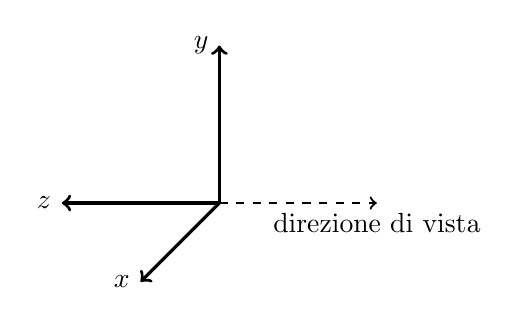
\begin{tikzpicture}[scale=2.0]
		\draw[dashed, thick, ->] (0.0, 0.0) -- (1.0, 0.0) node[below, color=black] {direzione di vista};
		\draw[very thick, ->] (0.0, 0.0) -- (-1.0, 0.0) node[left, color=black] {$z$};
		\draw[very thick, ->] (0.0, 0.0) -- (0.0, 1.0) node[left, color=black] {$y$};
		\draw[very thick, ->] (0.0, 0.0) -- (-0.5, -0.5) node[left, color=black] {$x$};
	\end{tikzpicture}
\end{center}

Questa \`e tuttavia solo una convenzione. Il vero sistema di riferimento nel quale vive la nostra scena, \`e sempre il
frame canonico. Dunque, i valori che useremo per $z$, quando trattiamo i movimenti dell'osservatore, saranno invertiti
ma poi dovranno essere svolte le opportune conversioni per rendere le modifiche consistenti con il frame canonico.

\subsection{Costruire un frame di vista (VRF)}
Un \textbf{frame di vista} o \textbf{View Reference Frame} si costruisce indicando, come prima cosa, la direzione in cui
stiamo guardando (o un punto verso cui guardare), definendo cos\`i la nostra \emph{view direction}. In seguito definiamo
qual \`e il nostro \emph{up}, ossia verso e direzione lungo i quali si sviluppa l'asse $y$.

I due assi appena definiti potrebbero non essere ortogonali fra loro per qualche motivo. Ma noi vogliamo sempre lavorare
con un frame ortonormale per evitare deformazioni indesiderate della nostra geometria.

Per ottenere un frame ortonormale dobbiamo
\begin{enumerate}
	\item Normalizzare la direzione di vista
	      \[ z = \frac{view\_direction}{\| view\_direction \|} \]
	\item Normalizzare l'\emph{up}
	      \[ y' = \frac{up}{\| up \|} \]
	\item Calcoliamo
	      \[ x = y' \times z \]
	      che sar\`a ortogonale a $z$.
	\item Calcoliamo infine
	      \[ y = x \times z \]
	      per ottenere l'asse $y$ ortogonale sia a $x$ che a $z$.
\end{enumerate}
Se scegliessimo la nostra \emph{view direction} e il nostro \emph{up}, l'uno ortogonale all'altro, ci basterebbe
calcolare il prodotto vettoriale tra i due per ottenere l'ultimo asse e costruire direttamente un frame ortogonale.

Una volta ottenuto un frame di vista ortogonale abbiamo il problema che la relativa matrice converte le coordinate dal
VRF al frame canonico quando noi vogliamo l'inverso. Per ottenere il risultato sperato ci baster\`a applicare l'inversa
\[ V = VRF^{-1} \]
che chiameremo \textbf{view matrix}.


La view matrix \`e la matrice di trasformazione che si occupa di muovere il punto di vista lungo i tre assi del VRF.

Per creare questo effetto non dobbiamo fare altro che applicare delle trasformazioni al VRF, ma pensandole in maniera
inversa.

Per esempio, se ci spostassimo verso destra, vedremo l'oggetto davanti a noi spostarsi verso sinistra.
\begin{center}
	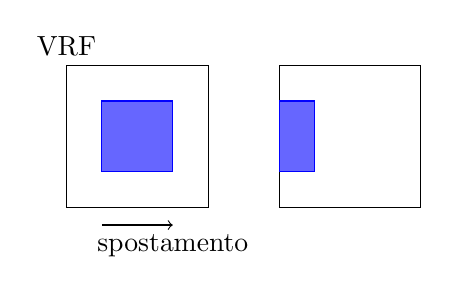
\begin{tikzpicture}[scale=0.45]
		\draw (-3, -3) --
		++ (0, 4) node[above] {VRF} --
		++ (4, 0) --
		++ (0, -4) --
		cycle;

		\draw [->] (-2, -3.5) -- ++(2, 0) node[below] {spostamento};

		\filldraw[draw=blue, fill=blue!60]
		(-2, -2) --
		++ (0, 2) --
		++ (2, 0) --
		++ (0, -2) --
		cycle;

		\draw (3, -3) --
		++ (0, 4) --
		++ (4, 0) --
		++ (0, -4) --
		cycle;

		\filldraw[draw=blue, fill=blue!60]
		(3, -2) --
		++ (0, 2) --
		++ (1, 0) --
		++ (0, -2) --
		cycle;
	\end{tikzpicture}
\end{center}
Per spostare quindi il punto di vista a destra, quello che dobbiamo fare in realt\`a, \`e spostare tutta la scena a
sinistra.

\section{Projection Matrix}
Mentre la view matrix si occupa di muovere il punto di vista nello spazio la \textbf{projection matrix} definisce il
tipo di camera che stiamo usando.

Ne esistono di due tipi, la prima \`e detta \textbf{prospettica}, la seconda invece \`e detta \textbf{ortogonale}.
Questi due tipi di camera creano due effetti distinti e si prestano per compiti abbastanza differenti.

\subsection{Perspective Projection}
La \textbf{matrice di proiezione prospettica}, come suggerisce il nome, serve a creare l'effetto della prospettiva.
Con questo tipo di camera noi andremo a definire una sorta di cono visivo a partire dal punto in cui \`e posizionata
la camera.

Questo \`e il tipo di camera che ci \`e pi\`u semplice immaginare dato che funziona esattamente come l'occhio umano:
gli oggetti che si allontanano ci appaiono pi\`u piccoli e quelli che che si avvicinano ci appaiono pi\`u grandi.
Si avr\`a inoltre un effetto prospettico molto simile a quello a cui siamo abituati.

\begin{center}
	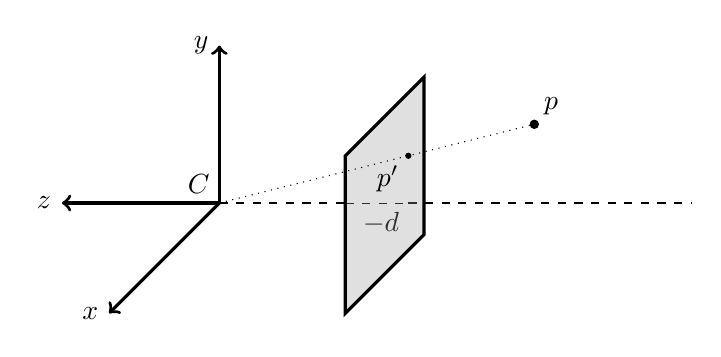
\begin{tikzpicture}[scale=2.0]
		\draw[dashed, thick] (0.0, 0.0) -- ++ (0.8, 0.0);
		\draw[dashed, ultra thin] (0.8, 0.0) -- ++ (0.4, 0.0) node[below left] {$-d$};
		\draw[dashed, thick] (1.2, 0.0) -- (3.0, 0.0);
		\draw[very thick, ->] (0.0, 0.0) -- ++ (-1.0, 0.0) node[left, color=black] {$z$};
		\draw[very thick, ->] (0.0, 0.0) -- ++ (0.0, 1.0) node[left, color=black] {$y$};
		\draw[very thick, ->] (0.0, 0.0) -- ++ (-0.7, -0.7) node[left, color=black] {$x$};

		\filldraw[very thick, fill=black!40, fill opacity=0.3]
		(0.8, 0.3) --
		++ (0, -1) --
		++ (0.5, 0.5) --
		++ (0, 1) --
		cycle;

		\coordinate (0, 0) node[above left] {$C$};

		\draw[dotted] (0.0, 0.0) -- ++ (2, 0.5);
		\fill (2, 0.5) circle[radius=0.03] node[above right] {$p$};
		\fill (1.2, 0.3) circle[radius=0.02] node[below left] {$p'$};
	\end{tikzpicture}
\end{center}
La figura rappresenta una prima parte di come funziona questo tipo di camera. In pratica dobbiamo immaginarci una
finestra (rappresentata dal quadrato grigio) attraverso la quale vediamo la scena.

L'osservatore si trova nel punto $C$ e tutto ci\`o che si trova tra il punto $C$ e la finestra non viene visto. Tutto
ci\`o che invece si pu\`o osservare si trova oltre la finestra.

Il punto $p$ verr\`a proiettato sulla finestra attraverso la linea tratteggiata che lo unisce con $C$. Il punto $p'$
sar\`a appunto la proiezione del punto $p$ sulla finestra.

Per capire quali siano le coordinate di $p'$ ci conviene vedere l'immagine di lato.
\begin{center}
	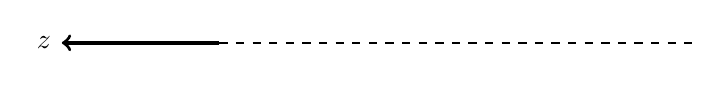
\begin{tikzpicture}[scale=2.0]
		\draw[very thick, ->] (0, 0) -- (-1, 0) node[left] {$z$};
		\draw[thick, dashed] (0, 0) -- (3, 0);
	\end{tikzpicture}
\end{center}